\newpage

\chapter{\textsc{Використання FHE в хмарних технологіях}}

\section{Бібліотека HeLib}
Для реалізації поставленої задачі буде використовуватись бібліотека гомоморфного шифрування
HeLib. HeLib була написана на С++ та реалізовує функціонал  Brakerski-Gentry-Vaikuntanathan 
(BGV), та Cheon-Kim-Kim-Song (CKKS) схем.

З середини 2018 року HElib знаходиться на стадії інтенсивного рефакторінгу для підвищення
надійності, розширяємості, продуктивності та, найголовніше, легкості у використанні для дослідників та розробників, які працюють з HE та його застосуванням.

\subsection{Алгоритми над схемою}
todo:


\section{Реалізація застосунку}
Для демонстрації коректності роботи, та можливості застосування FHE схеми у хмарних 
технологіях, був реалізований клієнт-серверний застосунок. Застосунок повинен реалізовувати
логіку банківської системи, тобто клієнт повинен мати можливість створити рахунок,
додати баланс, та зняти баланс з рахунку. Окрім цього, система бути розроблена з розрахунком
на те що вона буде знаходитись на хмарі, та між клієнтом і хмарою буде незахищене з'єднання.
Також, користувач банківського сервісу хоче бути впевнений в повному захисті даних, в тому
числі від сервера. Для реалізації вимог для безпеки даних буде використана FHE з реалізацією
BGV схеми в бібліотеці HeLib. Див. Рис 2.1.

\begin{figure}[!ht]
    \centering
    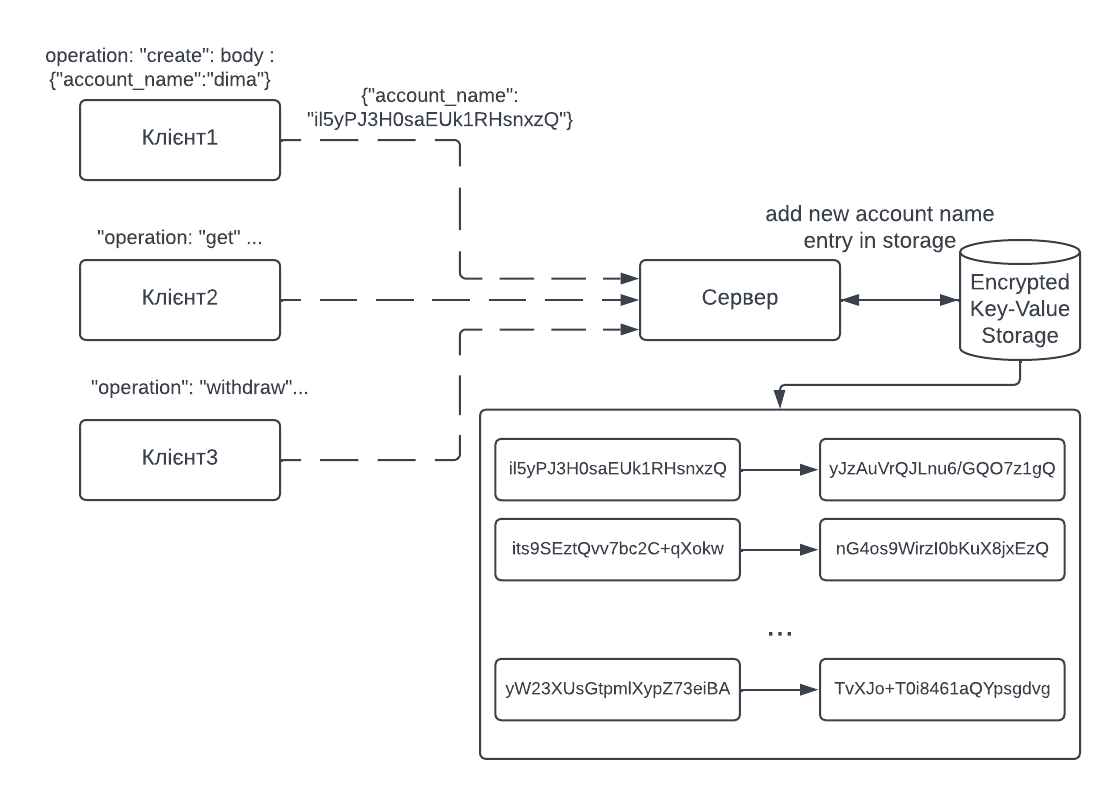
\includegraphics{static/client-server-logic.png}
    \caption{Демонстрація запитів клієнтів до серверу, де перервана стрілочка, означає
    незахищене середовище, тому данні в ньому будуть зашифровані}
    \label{fig:client-server-logic}
\end{figure}

\subsection{Вимоги}
Ця секція описує вимоги до розробки банківської системи, яка повинна забезпечувати коректність,
та безпеку даних.
\subsubsection*{Клієнт}
Основна задача клієнта, це створити необхідний контекст для FHE шифрування, ініціювати
з'єднання з сервером, робити необхідні запити, та обробляти відповіді від сервера.

Як було написано вище, клієнт повинен бути відповідальний за створення контексту шифрування. Під
контекстом, будемо вважати необхідні дані для правильного працювання FHE, зашифровування та розшифровування даних.
Деяку частину контекста необхідно буде надати серверу для того, щоб він мав можливість виконувати
розрахунки над зашифрованими даними, проте частина контекста повинна бути нерозголошуєма, така як
приватний ключ.

Контекст буде зберігатись на машині клієнта у файлі Json формату, і при ініціюванні з'єднання
з сервером, у клієнта повинна бути можливість вибору, чи створювати новий контекст, чи використати
присутній.

Нехай контекст був згенерований з деякими тестовими параметрами тоді його Json, та приватний
ключ буде виглядати наступним чином:

\begin{lstlisting}[breaklines, caption={Json репрезентація, контексу, деякі довгі послідовносиі чисел були замінені на трикрапку, щоб зменшити кількість тексту}, 
captionpos=b]
{"HElibVersion":"2.2.0","content":{"alsoThick":false,"build_cache":false,"digits":[[6,"..."],[11,"..."]],"ePrime_param":4,"e_param":12,"gens":[2341,3277,911],"hwt_param":120,"m":4095,"mvec":[7,"..."],"ords":[6,4,6],"p":2,"qs":[249047285761,"..."],"r":1,"scale":10.0,"smallPrimes":[0,"..."],"specialPrimes":[15,"..."],"stdev":{"exponent":0,"mantissa":3.2}},"serializationVersion":"0.0.1","type":"Context"}
\end{lstlisting}

\begin{lstlisting}[breaklines, caption={Json репрезентація приватного ключа}, captionpos=b]
{"HElibVersion":"2.2.0","content":{"b":[{"map":[[ large amount of 64-bits integers]],"set":[6,7,...]}]},"serializationVersion":"0.0.1","type":"SecKey"}
\end{lstlisting}
Клієнт повинен правильно серіалізувати свій контекст, для подальшого відправлення серверу,
та приватний ключ, для зберігання.

\begin{lstlisting}[breaklines, caption={Json формат зберігання приватного контексту на 
клієнті, для можливості його подальшого використання}, captionpos=b]
{
    "public_context": "Listing 2.1",
    "private_key": "Listing 2.2"
}
\end{lstlisting}

\subsubsection*{Сервер}
Задача серверної частини застосунку, це приймати TCP/IP з'єднання, та коректно обробляти 
запити від клієнта. Окрім глобальної задачі сервера, він повинен виконувати якусь логіку.

Також для зручного використання на хмарі, сервер повинен мати інструмент автоматичної розгортки,
для цього буде використана технологія контейнеризації Docker.

Фактично, логіку серверу можна поділити на 2 частини:
\begin{itemize}
    \item{\textbf{Пошук сутності в зашифрованій базі даних}: Хоча задача пошуку даних в базі
даних, може здатись тривіальною задачею, коли сервер працює повністю над зашифрованими даними,
задача стає дещо складнішою, оскільки шифрування одних і тих самих даних, може давати різний
результат кожен раз, тому просте зіставлення з даними в базі не дасть коректного результату.

Для коректного знаходження даних в базі, за ключем буде використовуватись наступний алгоритм:

Нехай у нас є сховище ключ-значення Рис. 2.2.


\begin{figure}[!ht]
    \centering
    \label{fig:key-value-storage}
    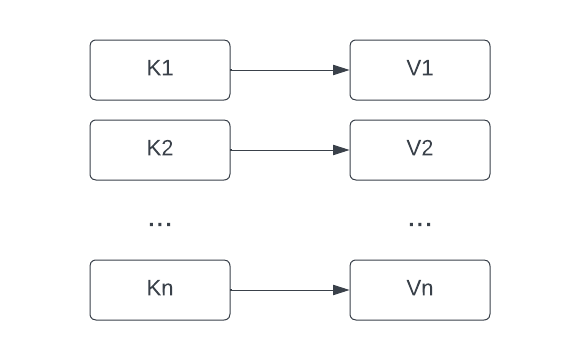
\includegraphics[scale=1.25]{static/key-value-storage.png}
    \caption{Де \(K\)- це множина ключів, та \(k_1,k_2,...,k_n \in K\), \(v_1, v_2,...,v_n 
    \in V\), де \(V\)- це множина значень, а \(n\)-кількість сутностей в базі. Тобто
    відображення \(K \rightarrow V\) є бієктивним.}
\end{figure}

    Високорівнево, алгоритм пошуку в базі, над зашифрованими даними описаний на заображенні
    Рис. 2.3.

\begin{figure}[!ht]
    \label{fig:basic-value-extraction}
    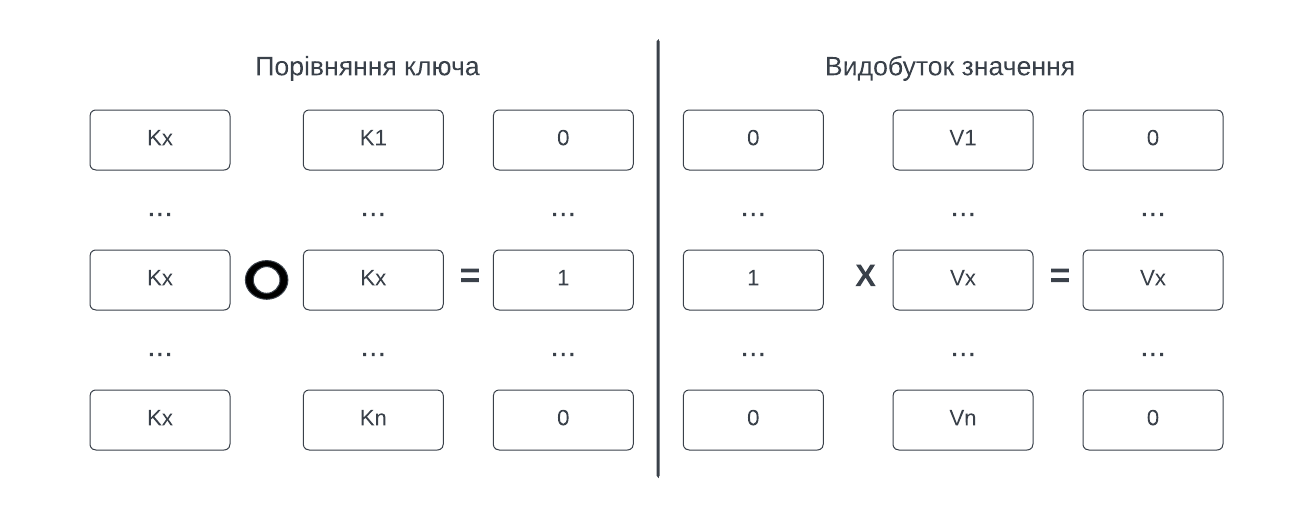
\includegraphics[scale=0.85]{static/basic-value-extraction.png} 
    \caption{Спрощений алгоритм пошука значення \(V_x \in V\), за ключем \(K_x \in K\)}
\end{figure}

    Далі буде описано більш детально алгоритм пошуку за ключем в зашифрованій базі даних.
    
    Першим кроком алгоритму є обчислення операції різниці між запитом і ключами бази даних. Це
    проста операція віднімання, яка поелементно виконує віднімання у структурі, схожій на масив. В
    результаті буде отримано різницевий шифротекст, який ми позначимо як \(\Delta_i\) де
\(\Delta_1,\Delta_2,...,\Delta_n \in \delta\). Наразі 
    \(\Delta = 0\) якщо \(k_q \in K\), і ненульовому значенню в іншому випадку, див. Рис. 2.4.

\begin{figure}[!ht]
    \centering
    \label{fig:key-subsruction}
    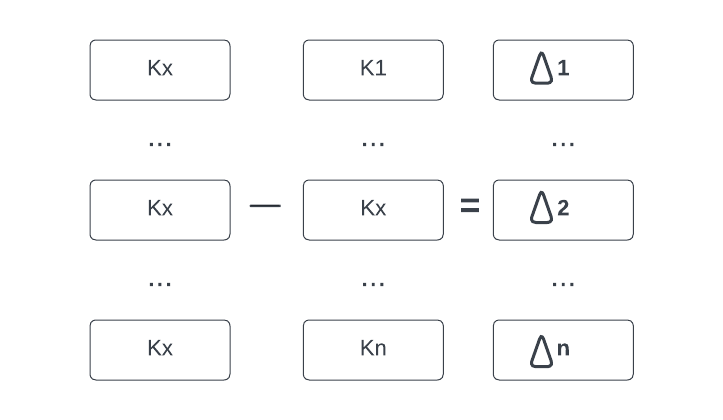
\includegraphics[scale=1.25]{static/key-substruction.png}
    \caption{Віднімання ключів, щоб отримати \(\Delta_1,\Delta_2,...,\Delta_n \in \delta\).
    Де у випадку \(K_q \in K\, \Delta_q = 0, \Delta_i \neq 0, i \neq q\)}.
\end{figure}


Це не зовсім та маска, яка нам потрібна, тому ми повинні виконати іншу операцію, описану далі.
Для отримання правильної маски, треба буде застосувати малу теорему Фермa  \cite{Fermat} до
\(\Delta_i \in \delta\). Застосувавши теорему, ми отримаємо наступний результат:

\begin{align*}
\text{LTF}(\Delta_i) =
\begin{cases} 
    1, & \Delta_i \neq 0 \\
    0, & \Delta_i = 0
\end{cases}
\end{align*}

Проте, ця маска дає обернений результат, щоб отримати коректні значення, треба застосувати
операцію інверсії:

\begin{align*}
1- \text{LTF}(\Delta_i) =
\begin{cases} 
    0, & \Delta_i \neq 0 \\
    1, & \Delta_i = 0
\end{cases}
\end{align*}

Якщо описати процес знаходження над зашифрованими даними \textsc{\textbf{enc}}(\(x\)), то це
буде виглядати так, як зображено на Рис. 2.5.

Спочатку ми застосовуємо операцію малої теореми Ферма (FLT) \cite{Fermat} до кожного різницевого
зашифрованого тексту. Це призводить до шифрування нуля, \(E(0)\), якщо різниця дорівнює нулю,
тобто є збіг, і шифрування одиниці, \(E(1)\), в іншому випадку.

Далі ми використовуємо попередньо обчислені результати операції FLT і віднімаємо це значення від
1. Це значення 1 може бути чистим, оскільки будь-яка операція між зашифрованим текстом і
відкритим текстом призводить до зашифрованого тексту. Це призводить до відображення будь-якого
ненульового значення в нуль і нуля в одиницю. Таким чином, ми отримуємо маски, які нам потрібні
для алгоритму порівняння. 

Однак є ще один аспект, який слід взяти до уваги, а саме: як ми повинні діяти з частковими збігами?

\begin{figure}[!ht]
    \centering
    \label{fig:mask-creation-flow}
    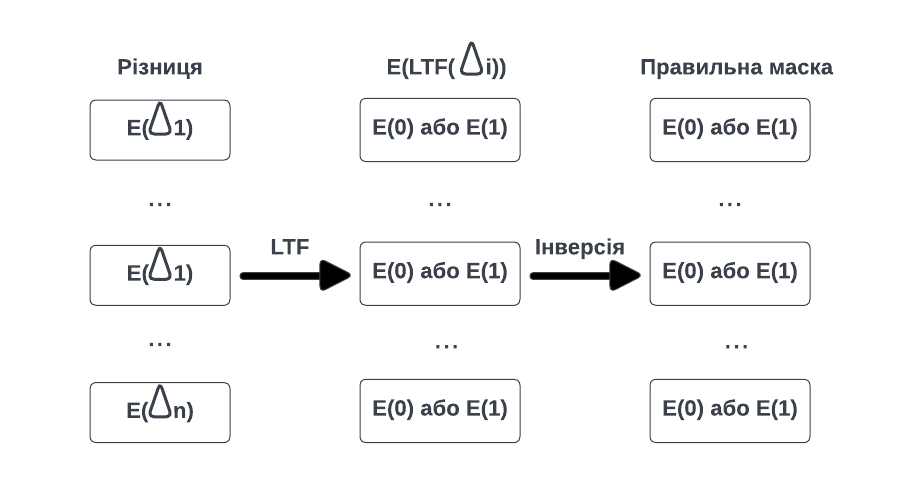
\includegraphics[scale=1.25]{static/mask-creation-flow.png}
    \caption{Процес створення правильної маски над зашифрованими даними}
\end{figure}
Розглянемо наступний сценарій, показаний на зображенні нижче Рис 2.6. Уявіть, що ключ збігається лише з
другою літерою запиту і, можливо, з деякими значеннями пропусків, тоді він створить масив, як
показано нижче Рис. 2.6.

Оскільки в нашому прикладі нас цікавлять лише точні збіги, цей результат слід вважати таким, що
не збігається. Щоб усунути часткові збіги, ми просто копіюємо зашифрований текст, виконуємо
обертання структури масиву в копії і перемножуємо його за входом з оригінальною копією. Це
означає, що якщо в одному з осередків зашифрованого тексту є хоча б один 0, то цей осередок
ефективно обнулить всі інші осередки масиву.

Зауважте, що оскільки ми не можемо знати, який саме шифротекст містить результат, що збігається,
частково збігається або не збігається, ця операція також виконується над результатом, що
збігається. Однак, оскільки у зашифрованому тексті у кожному слоті має бути 1, то ця операція не
повинна мати ніякого ефекту.

\begin{figure}[!ht]
    \centering
    \label{fig:partial-match}
    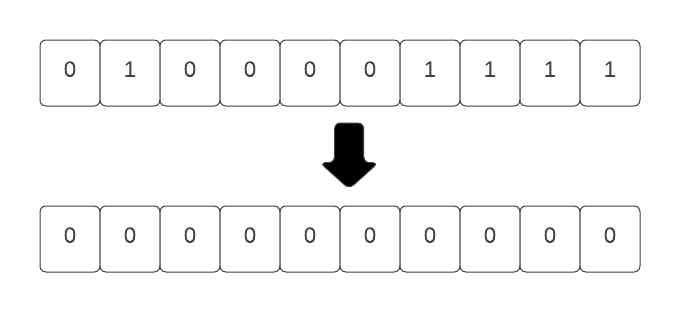
\includegraphics{static/partial-match.png}
    \caption{Частковий збіг, який не повинен вважатись коректним}
\end{figure}

Тепер, коли ми маємо остаточні маски, ми можемо виконати вилучення даних з бази даних. Цей крок
передбачає множення маски на відповідний запис у базі даних. Оскільки наша маска є шифруванням 0,
якщо немає збігу, множення її на відповідний запис обнулить цей запис. Крім того, оскільки маска
є шифруванням 1, якщо є збіг, множення її на запис поверне сам запис. 

Оскільки ключі в нашому прикладі бази даних є унікальними, можна бути впевненим, що на кожен
запит буде отримано максимум один унікальний збіг. Використовуючи ці знання, можна об'єднати всі
результати кроку вилучення значень в один зашифрований текст. Це пов'язано з тим, що додавання
шифрів 0 до значення не змінює саме значення. Це дозволяє економити на зв'язку, оскільки серверу
потрібно надсилати клієнту лише один зашифрований текст, а не по одному зашифрованому тексту для
кожного запису в базі даних.

}
    \item{\textbf{Виконання розрахунків над зашифрованими даними}:}
\end{itemize}


\subsubsection*{Комунікація клієнту з сервером (API)}
Клієнт повинен мати можливість комунікувати з сервером і робити запит на операції: створити
новий рахунок, зняти баланс з рахунку, додати баланс на рахунок, та отримати інформацію
про кількість грошей на рахунку. Окрім цього, для деяких операцій, клієнт повинен надати
серверу деякі дані, наприклад під час створення рахунку, клієнт повинен відправити FHE контекст
для того, щоб сервер міг правильно працювати з цими даними в майбутньому.

Для спрощення імплементації, клієнт буде відправляти та отримувати дані в форматі Json, в
якому буде міститись поле про тип операції (create, get, add, withdraw) в полі 
request (запит), та необхідну інформацію в полі body (тіло).

Також як було описано в Ліст. 2.1. клієнт відповідальний за відправку FHE контексту шифрування,
щоб забезпечити можливість серверу коректно працювати з даними клієнта. Важливо зазначити, що
цей контекст не дає можливість розшифровувати данні.

\subsection{Стек технологій для розробки}
Для реалізації банківської системи був вибраний наступний стек технологій:
\begin{itemize}

    \item{Мова розробки була вибрана: C++, так як реалізація FHE схем краще всього написана
на ній і показують достойну швидкість обчислення}
    \item{Для реалізації FHE буде використана бібліотека з відкритим кодом HeLib, з
якої буде взята логіка BGV схеми}
    \item{Для TCP/IP з'єднання між клієнтом та сервером (хмарою) буде використана бібліотека
з колекції Boost: Asio, яка дозволяє виконувати асинхронні операції з IO девайсами, в тому
числі в ній знаходиться функціонал для реалізації TCP/IP з'єднань.}
    \item{Для більш зручної розробки будуть використані сторонні бібліотеки та інструменти:
логування, збірка проєкту, тестування, засоби вимірювання швидкодії.}
\end{itemize}


